\section{Graph Modeling}
Quando si parla di \textbf{Data Modeling} si intende il processo per cui una entitá reale di qualunque tipo viene trasformata nel suo corrispondente software. La misura in cui otteniamo rappresentazioni software accurate di questi elementi del mondo reale determina l'efficacia con cui affrontiamo il problema previsto. Suddividiamo il problema in 4 steps: 
\begin{itemize}
    \item \textbf{Capire il problema}: specificando i termini comuni e i principali modelli di accesso degli utenti ovvero come verranno fatte le query (core access pattern), le informazioni principali, ecc...
    \item \textbf{Creare un modello concettuale}: disegnare un diagramma che descriva in maniera approssimativa il problema da un punto di vista non tecnico e implementativo dal punto di vista degli obiettivi, delle esigenze e delle operazioni dell'organizzazione.
    \item \textbf{Creare un modello logico}: definire i vertici e gli archi con le loro proprietá.
    \item \textbf{Testare il modello}: verificare che il modello creato soddisfi il problema, che esistano le risposte alle nostre domande. 
\end{itemize}

\subsection{Capire il problema}
Vediamo una serie di domande che possono far capire chiaramente il tipo di problema:
\begin{itemize}
    \item Cosa deve fare il grafo per l'utente? (Dominio e scopo)
    \item Quali sono i building blocks fondamentali del nostro progetto? Come sono collegati tra loro? (Business entity)
    \item Come verrá usato il sistema? (Functionality)
\end{itemize}

\paragraph{Esempio} Vediamo come applicare queste domande a \textbf{DiningByFriends}, applicazione per raccomandazioni gastronomiche. 
\begin{quote}
    Domanda 1: Cosa deve fare il grafo per l'utente?
\end{quote}
DiningByFriends crea una lista di posti suggeriti dove mangiare personalizzata per l'utente. Deve quindi garantire che:
\begin{itemize}
    \item ci si possa connettere con amici che usano l'applicazione
    \item si possa creare recensioni di piatti e ristoranti
    \item mettere un rating alle recensioni per capire quanto sono inerenti o importanti
\end{itemize}
\begin{quote}
    Domanda 2: Quali sono i building blocks fondamentali del nostro progetto? Come sono collegati tra loro?
\end{quote}
Sicuramente servirá un'autenticazione dell'utente, e i dati di tutti i ristoranti. Servirá tenere le recensioni, i ratings sia dei commenti che dei locali, la lista degli amici ecc...
\begin{quote}
    Domanda 3:  Come verrá usato il sistema? 
\end{quote}
Tante le funzionalitá da tenere a mente, gli amici, i likes, i voti, i ristoranti... E poi fare classifiche, categorie, e molto altro.

\newpage

\subsection{Creare un modello concettuale}
Uno dei primi step nella creazione del modello concettuale, collegandoci sempre all'esempio precedente e avendo giá risposto a tutte le domande della prima fase, sará quello di definire le entities: sicuramente ristoranti, i menu, le persone e le recensioni. Poi, lo step successivo sará quello di identificare delle relazioni tra entities: 
\begin{itemize}
    \item relazione 1 potrebbe essere Persona-Amico-Persona
    \item relazione 2 potrebbe essere Persona-Scrive-Recensione 
\end{itemize}
La relazione tra le entities é ovviamente "amico" nel primo caso e "scrive" nel secondo. 
\\
\begin{figure}[th]
    \centering
    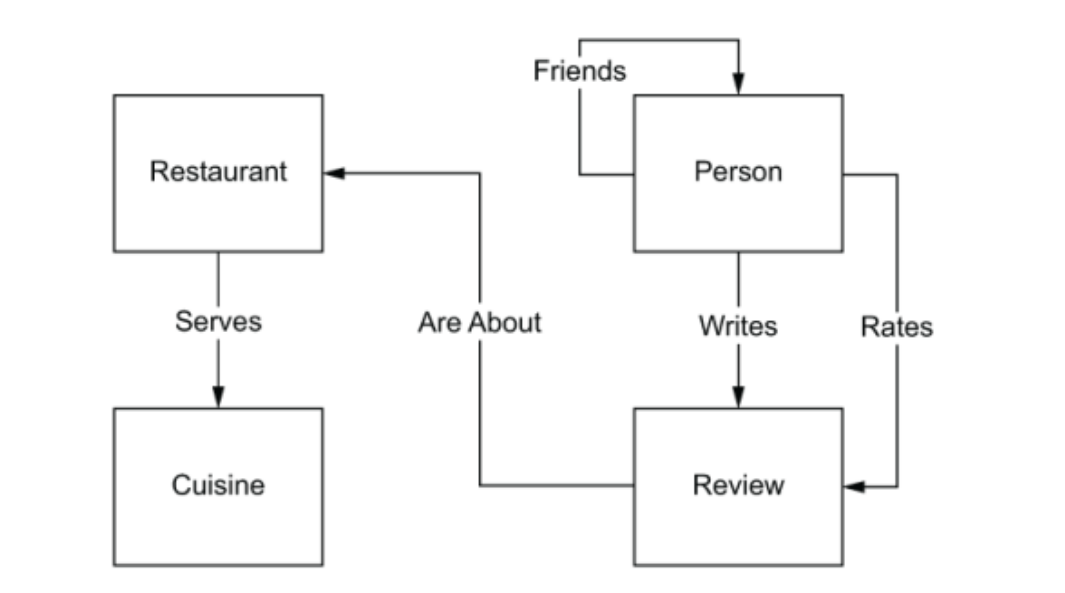
\includegraphics[width=0.5\linewidth]{GraphModeling//img/esempio.png}
\end{figure}

\subsection{Costruire un graph data model}
Per costruire il modello a grafo é necessario seguire questi passaggi: 
\begin{enumerate}
    \item Traduzione delle entitá in nodi (vertici)
    \item Traduzione delle relazioni in archi (edges)
    \item Assegnare le varie proprietá ad archi e vertici
    \item Fare un check finale del modello
\end{enumerate}

\subsubsection*{Step 1: Traduzione delle entitá in nodi}
Per la creazione dei vertici del modello abbiamo bisogno di due cose principalmente: \textbf{identificare} tutte le entities rilevanti dal conceptual model e \textbf{denominare} correttamente l'entity in modo che sia ben distinguibile all'interno del modello. 
\begin{quote}
    É best practice fare in modo che ogni label di ogni vertice sia singola poiché ogni vertice si riferisce ad una singola istanza di un elemento. 
\end{quote}

\subsubsection*{Step 2: Traduzione delle relazioni in archi}
Gli archi sono basati sulle relazioni trovate nel modello concettuale, ma per essere definite lo sforzo é maggiore rispetto ai vertici. Questo perché gli archi possiedono proprietá di \textbf{unicitá} e \textbf{direzione} che non hanno una diretta controparte nei database relazionali. Le operazioni da svolgere nel caso di archi sono infatti: \textbf{identificare} le relazioni rilevanti e \textbf{denominarle}; assegnare una \textbf{direzione} da un vertice ad un altro e \textbf{specificare} l'unicitá di tale arco definendo il numero di volte che puó esistere tra due diversi vertici (praticamente, specifichiamo quante volte questo tipo di relazione esiste). 

\paragraph{Esempio} Tornando a DiningByFriends, le domande che possono essere sorte nella fase di elaborazione del conceptual model, in particolare nella parte di social networking sono:
\begin{itemize}
    \item chi sono i miei amici?
    \item chi sono gli amici dei miei amici?
    \item come l'utente X é associato all'utente Y?
\end{itemize}
Tutte queste domande dipendono dal tipo di \textbf{relazione} tra due persone. Quindi \textbf{Amicizia} sará sicuramente un edge nel mio grafo, e collegherá due vertex \textbf{Persona}. 
\\
Ora che abbiamo deciso che dev'essere un arco, lo denominiamo "friend" e otteniamo una struttura di questo tipo: 
\\
\begin{figure}[th]
    \centering
    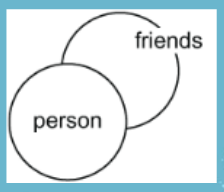
\includegraphics[width=0.25\linewidth]{GraphModeling//img/friend.png}
\end{figure}
\\
Il prossimo passaggio sará quello di assegnargli una direzione, definendo un vertex di uscita e uno di ingresso, e stabilendo che:
\begin{quote}
    Se Marco $\rightarrow$ Daniele, Marco é amico di Daniele 
\end{quote}
E quindi Daniele é nella sua lista degli amici. Da slide: in un buon graph model, gli archi devono leggersi come frasi. Graficamente parlando:
\\
\begin{figure}[th]
    \centering
    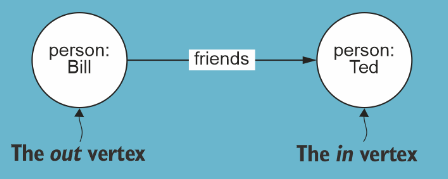
\includegraphics[width=0.5\linewidth]{GraphModeling//img/billfriendsted.png}
    \caption{Bill é amico di Ted}
\end{figure}

\newpage

Ora viene lo step piú complicato, assegnare l'\textbf{unicitá} di un edge, che descrive il numero di volte che due vertici vengono connessi da un arco che ha lo stesso nome (guardando l'immagine sopra, quante volte usi l'arco friends). 
\\
\begin{figure}[th]
    \centering
    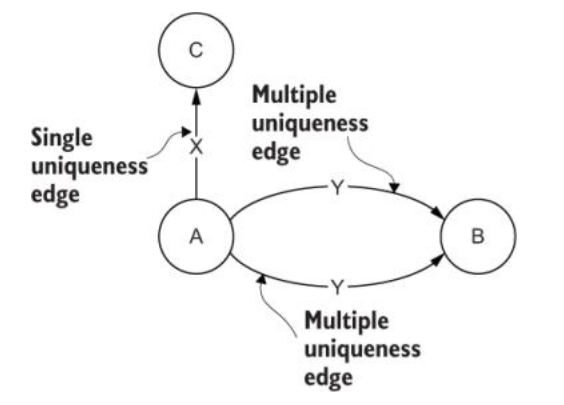
\includegraphics[width=0.5\linewidth]{GraphModeling//img/uniqueness.png}
\end{figure}
\\
\textbf{Perché si parla di uniqueness e non di cardinality o multiplicity?} Quando si parla di metodi di modellazione dei dati, il termine cardinalità viene usato per indicare quante entità possono essere collegate tra loro. Ad esempio, si può avere una relazione tra ordine e cliente e dire che la cardinalità della relazione è uno-a-molti. Oppure si può dire che la cardinalità dei clienti per un ordine è zero-a-molti. \\
L’UML (Unified Modeling Language) evita il termine cardinalità, preferendo usare il termine molteplicità (multiplicity). Spesso, chi proviene da un background di modellazione dei dati ne rimane sorpreso, poiché il termine cardinalità è stato largamente usato in quel contesto. \\
Il motivo di questo cambiamento è che, secondo la definizione del dizionario, la cardinalità è “il numero di elementi in un insieme o altro raggruppamento” (Oxford English Dictionary). In base a questa definizione, l’uso del termine cardinalità nella modellazione dei dati sarebbe in realtà scorretto. Nel suo eccellente UML Reference Manual, Rumbaugh definisce la molteplicità come “una specifica dell’intervallo di valori ammissibili di cardinalità – cioè la dimensione – che un insieme può assumere”. L’UML utilizza la molteplicità in vari contesti: per una proprietà (associazione o attributo) e anche per mostrare la molteplicità delle parti in una struttura composita. È formalmente definita come un limite inferiore e uno superiore. Un’associazione (l’equivalente UML di una relazione nella modellazione dei dati) ha una molteplicità per ciascuna direzione. 
\newpage
\paragraph{Definizione} Si parla di \textbf{Multiple uniqueness} quando l'arco che collega tra loro due vertici si ripete piú volte. 
\\
\begin{figure}[th]
    \centering
    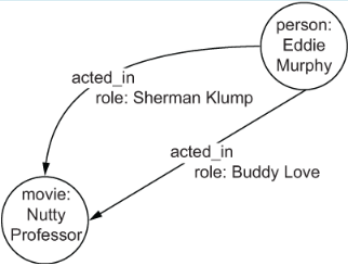
\includegraphics[width=0.35\linewidth]{GraphModeling//img/multipleuniq.png}
\end{figure}
\\
Questo é un chiaro esempio di multiple uniqueness, quando viene collegato Eddie Murphy a due ruoli nel film \textit{Il professore matto}. Il problema di una uniqueness errata puó essere davvero deleterio per un sistema:
\begin{itemize}
    \item se abbiamo edges single unique, ma che dovrebbero essere multipli
    \item se abbiamo edges multiple unique, ma che dovrebbero essere singoli
    \item inoltre una query fará piú fatica a ritornare tutti i risultati nel caso di una multiple uniqueness
\end{itemize}
\begin{figure}[th]
    \centering
    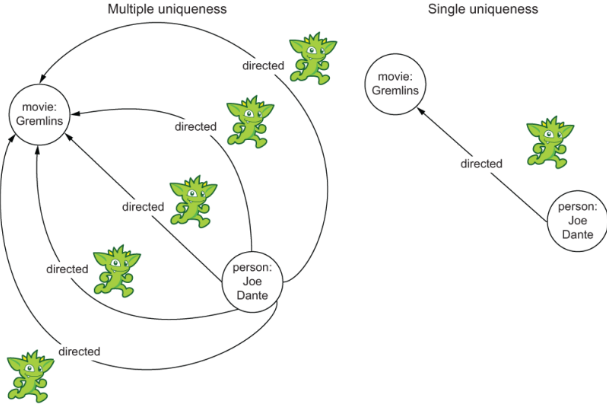
\includegraphics[width=0.75\linewidth]{GraphModeling//img/issues.png}
\end{figure}

\newpage
\subsubsection*{Step 3 : Assegnare proprietá a vertici e nodi}
Le proprietá in un grafo sono coppie chiave valore che descrivono un attributo specifico di un vertex o un edge. Le principali domande da porsi quando devono essere assegnate delle proprietá sono: 
\begin{itemize}
    \item che proprietá sono richieste?
    \item che nome gli diamo?
    \item qual é il loro data type?
\end{itemize}
Per rispondere a tali domande bisogna fare riferimento al modello concettuale preparato e vedere quali dati vanno salvati. 

\paragraph{Esempio} Guardando sempre il nodo "Persona" e arco "Amico", le domande sono sempre le stesse:
\begin{itemize}
    \item chi sono i miei amici?
    \item chi sono gli amici dei miei amici?
    \item come l'utente X é associato all'utente Y?
\end{itemize}
Quindi sappiamo che sicuramente abbiamo bisogno di dare un nome ed un cognome ad ogni Persona e che possiamo inserirli come \textbf{proprietá}. Poi sicuramente servirá un identificatore unico per ogni persona, un id, per distinguere vari omonimi quando si vuole creare un collegamento di amicizia. 
\\
\begin{figure}[th]
    \centering
    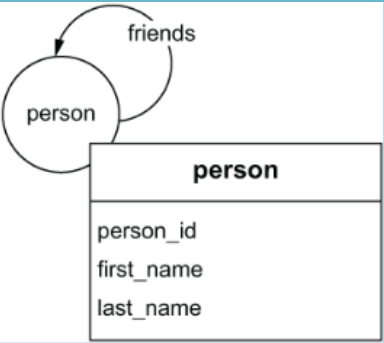
\includegraphics[width=0.25\linewidth]{GraphModeling//img/properties.png}
\end{figure}
\\
\paragraph{Bivio} A questo punto se decidi di usare un qualunque graph model schemaless che esiste sul mercato, hai finito. Invece se ti é necessario esplicitare lo schema hai ancora uno step da fare: tradurre il tuo logical data model nel physical data model richiesto dal database scelto. 
\\
Quando progetti un sistema, prima crei un modello logico dei dati – cioè una rappresentazione concettuale di come i dati sono organizzati e come sono collegati (per esempio: “Un cliente può fare più ordini”). Ma ogni database ha le sue regole per come quei dati devono essere effettivamente memorizzati. Questo si chiama modello fisico dei dati.
\\
Due casi possibili:
\begin{enumerate}
    \item Stai usando un database "schemaless" (senza schema fisso): \\
    Alcuni database a grafo, come Neo4j o altri NoSQL, ti permettono di non specificare lo schema in anticipo. Puoi semplicemente iniziare a inserire dati, e il database li accetta così come sono. $\rightarrow$ In questo caso sei a posto, non devi fare altro.
    \item Stai usando un database che richiede schema esplicito (ad esempio, un RDBMS come PostgreSQL o un grafo con schema fisso): \\
    Qui devi specificare in dettaglio quali sono i nodi, le relazioni, le proprietà, i tipi di dati ecc.
    $\rightarrow$ Devi convertire il tuo modello logico (di concetti generali) in un modello fisico (concrete tabelle, colonne, tipi, vincoli...).
\end{enumerate}
    
\subsubsection*{Step 4: Fare un check finale del modello}
L'ultimo step nel create il nostro data model é quello di testare se possiamo dare una risposta alle domande prefissate in fase di progettazione. 
\paragraph{Esempio} Le domande:
\begin{itemize}
    \item chi sono i miei amici? Possiamo rispondere partendo dal nodo di una persona specifica trovata tramite id unico e attraversando tutti gli edge "Amico" che partono da questa persona. 
    \item chi sono gli amici dei miei amici? Partendo sempre da una persona specifica con il suo id, itero il processo ogni volta che raggiungo un amico guardo i suoi amici. 
    \item come l'utente X é associato all'utente Y? Cerchiamo partendo dall'id dell'utente X di arrivare, attraversando tutti gli edges possibili, all'utente Y.
\end{itemize}

\paragraph{Best practice} Alcuni controlli aggiuntivi di buone pratiche per assicurarci che il nostro modello di dati rappresenti un solido modello a grafo:

\begin{itemize}
  \item I vertici e gli archi si leggono come una frase? Sì. Anche se non è un requisito assoluto, è un ottimo controllo generale per verificare che le etichette dei vertici rappresentino i nomi nel tuo modello e che le etichette degli archi descrivano le azioni o i verbi.
  
  \item Ho etichette di vertici o archi diverse con le stesse proprietà? No. In questo caso, vogliamo solo una singola etichetta di vertice e una singola etichetta di arco.
  
  \item Il mio modello ha senso? Sì. Anche se questo passaggio può sembrare un controllo ovvio, vale la pena prendersi il tempo per fare un passo indietro e verificare che il tuo modello di dati a grafo non si sia allontanato troppo dal modello concettuale e che abbia senso per il problema che stai cercando di risolvere.
\end{itemize}
A tutto questo va aggiunta una fase di testing per capire se effettivamente sono necessarie altre funzionalitá, se quelle giá presenti possono essere modificate, se servono nuove proprietá ecc...